
\documentclass[a4paper, 12pt]{article}


\usepackage[czech]{babel}
\usepackage[utf8]{inputenc}
\usepackage[left=2cm, text={17cm, 24cm}, top=3cm]{geometry}
\usepackage{times}
\usepackage{verbatim}
\usepackage{enumitem}
\usepackage{graphicx}
\usepackage{amsthm, amsmath, amssymb}
\usepackage[unicode]{hyperref}
\usepackage{pdfpages}


\begin{document}


% Titulní stránka %

	\begin{titlepage}
		\begin{center}
			
\includegraphics[width=0.77\linewidth]{FIT_logo.pdf} \\

			\vspace{\stretch{0.382}}

			\Huge{Projektová dokumentace} \\
			\LARGE{\textbf{Implementace překladače imperativního jazyka IFJ20}} \\
			\Large{Tým 75, varianta 1}
			
		\end{center}
        \begin{center}
	            \Large{Implementovaná rozšíření: \textbf{BASE}}
	            \vspace{\stretch{0.618}}
		\end{center}
		\begin{minipage}{0.4 \textwidth}
			{\Large \today}
		\end{minipage}
		\hfill
		\begin{minipage}[r]{0.6 \textwidth}
			\Large
			\begin{tabular}{l l l}
				\textbf{Michal Pyšík} & (xpysik00) & \quad 25\,\% \\
				Karel Jirgl & (xjirgll00) & \quad 25\,\% \\
				Václav Klem & (xklem00) & \quad 25\,\% \\
				Thanh Quang Tran & (xtrant02) & \quad 25\,\% \\
			\end{tabular}
		\end{minipage}
	    
	\end{titlepage}

\tableofcontents

\newpage


\section{Spolupráce v týmu}
\subsection{Rozdělení práce v týmu}
Rozdělení práce probíhalo v době plánování. Nakonec jsme si všichni v různých částech implementace pomáhali, aby nebyl problém spojit všechny části předkladače v jeden funkční celek. Shodli jsme se na rovnoměrném rozdělení bodů, jelikož všichni členové týmu spolu aktivně komunikovali, pomáhali si a nebyly žádné významné neshody. 

\subsubsection*{Michal Pyšík (xpysik00)}
Implementace lexikálního analyzátoru a ustanovení typů tokenů

\subsubsection*{Karel Jirgl (xjirgl00)}
Gramatika, Syntaktická a sémantická analýza, implementace tabulky symbolů, LL tabulky, precedenční~syntaktické analýzy

\subsubsection*{Václav Klem (xklemv00) }
Generátor cílového kódu

\subsubsection*{Thanh Quang Tran (xtrant02)}
Gramatika, LL tabulka, tabulka precedenční syntaktické analýzy 

\subsubsection*{Společná práce}
Dokumentace, obecná struktura cílového programu

\subsection{Způsob práce v týmu}
Komunikace probíhala především prostřednictvím Discord serveru vytvořeného přímo pro tento projekt. Konaly se pravidelné porady a všichni členové týmu byli většinou k dispozici, pokud se vyskytl nějaký problém nebo bylo potřeba se dohodnout na konkrétních detailech implementace. Díky úspěšné komunikaci a vzájemnému porozumnění kódu mezi kolegy nebyl problém spojit jednotlivé části tak, aby spolu byly vzájemně kompatibilní. Pro správu zdrojových souborů jsme používali verzovací systém Git, většina práce se odehrávala pouze v hlavní větvi, jelikož v konkrétním souboru prováděla změny většinou jen jedna osoba najednou.

\newpage

\section{Lexikální analýza}
První částí překladače je lexikální analyzátor (scanner). Nejdůležitější funkcí je zde \verb|scannerGetToken|, což je vlastně implementace deterministického konečného automatu, který čte jednotlivé znaky ze standartního vstupu, dokud nedojde do koncového stavu (návratová hodnota 0), nebo nenarazí na lexikální chybu (návratová hodnota 1). To je zajištěné pomocí přepínače \verb|switch| umístěného v nekonečném \verb|while| cyklu, kde každý \verb|case| reprezentuje právě jeden stav automatu, a při každém opakování cyklu je čten právě jeden znak ze vstupu.
\newline
\newline
Funkce má jediný parametr, a to ukazatel na předem alokovaný prvek typu \verb|Token|, jehož typ (a případně atribut) se nastaví podle přečtených hodnot a dosaženého koncového stavu. Mezi typy tokenů bez atributů patří například relační operátory, aritmetické operátory, přiřazení, klíčová slova, odřádkování (\verb|EOL|), konec souboru (\verb|EOF|), závorky a další povolené znaky.
\newline
\newline
Typy tokenů s atributy jsou pouze identifikátor, celé číslo, desetinné číslo a řetězec. Atribut tokenu je typu \verb|union|, v případě identifikátoru nebo řetězce se tedy využívá pouze atribut \verb|string|, u celého čísla \verb|integer| a u desetinného čísla \verb|real|. Když je zřejmé že načítáme nějaký z těchto 4 typů tak se přečtené znaky nejprve ukládají do bufferu (globální pole), a ve chvíli kdy je dosaženo koncového stavu, se do následující pozice v bufferu vloží nulový znak. Obsah bufferu až po tento znak je poté převeden na celé/desetinné číslo, nebo zkopírován do nově alokovaného stringu (jehož velikost pro alokaci je index pozice prvního nulového znaku v bufferu + 1). Tento postup je velice praktický, protože i když se obsah bufferu nemaže ale pouze přepisuje, cokoli za prvním nulovým znakem je ignorováno, například pozůstatky nějakého delšího dříve načteného řetězce. V případě ID se ještě zavolá funkce \verb|keywordCheck|, která kontroluje zda se nejedná o klíčové slovo, v takovém případě uvolní alokovaný \verb|string| a nastaví odpovídající typ tokenu.
\newline
\newline
Všechny načtené tokeny se ukládají do obousměrně vázaného lineárního seznamu \verb|tokenList|, který je předáván dalším částem překladače. Z pracujících se seznamem stojí za zmínku \verb|ScannerGetTokenList|, která plní seznam tokeny (voláním dříve popsané funkce), dokud nenarazí na token typu \verb|EOF|, nebo volaná funkce nenahlásí lexikální chybu. 


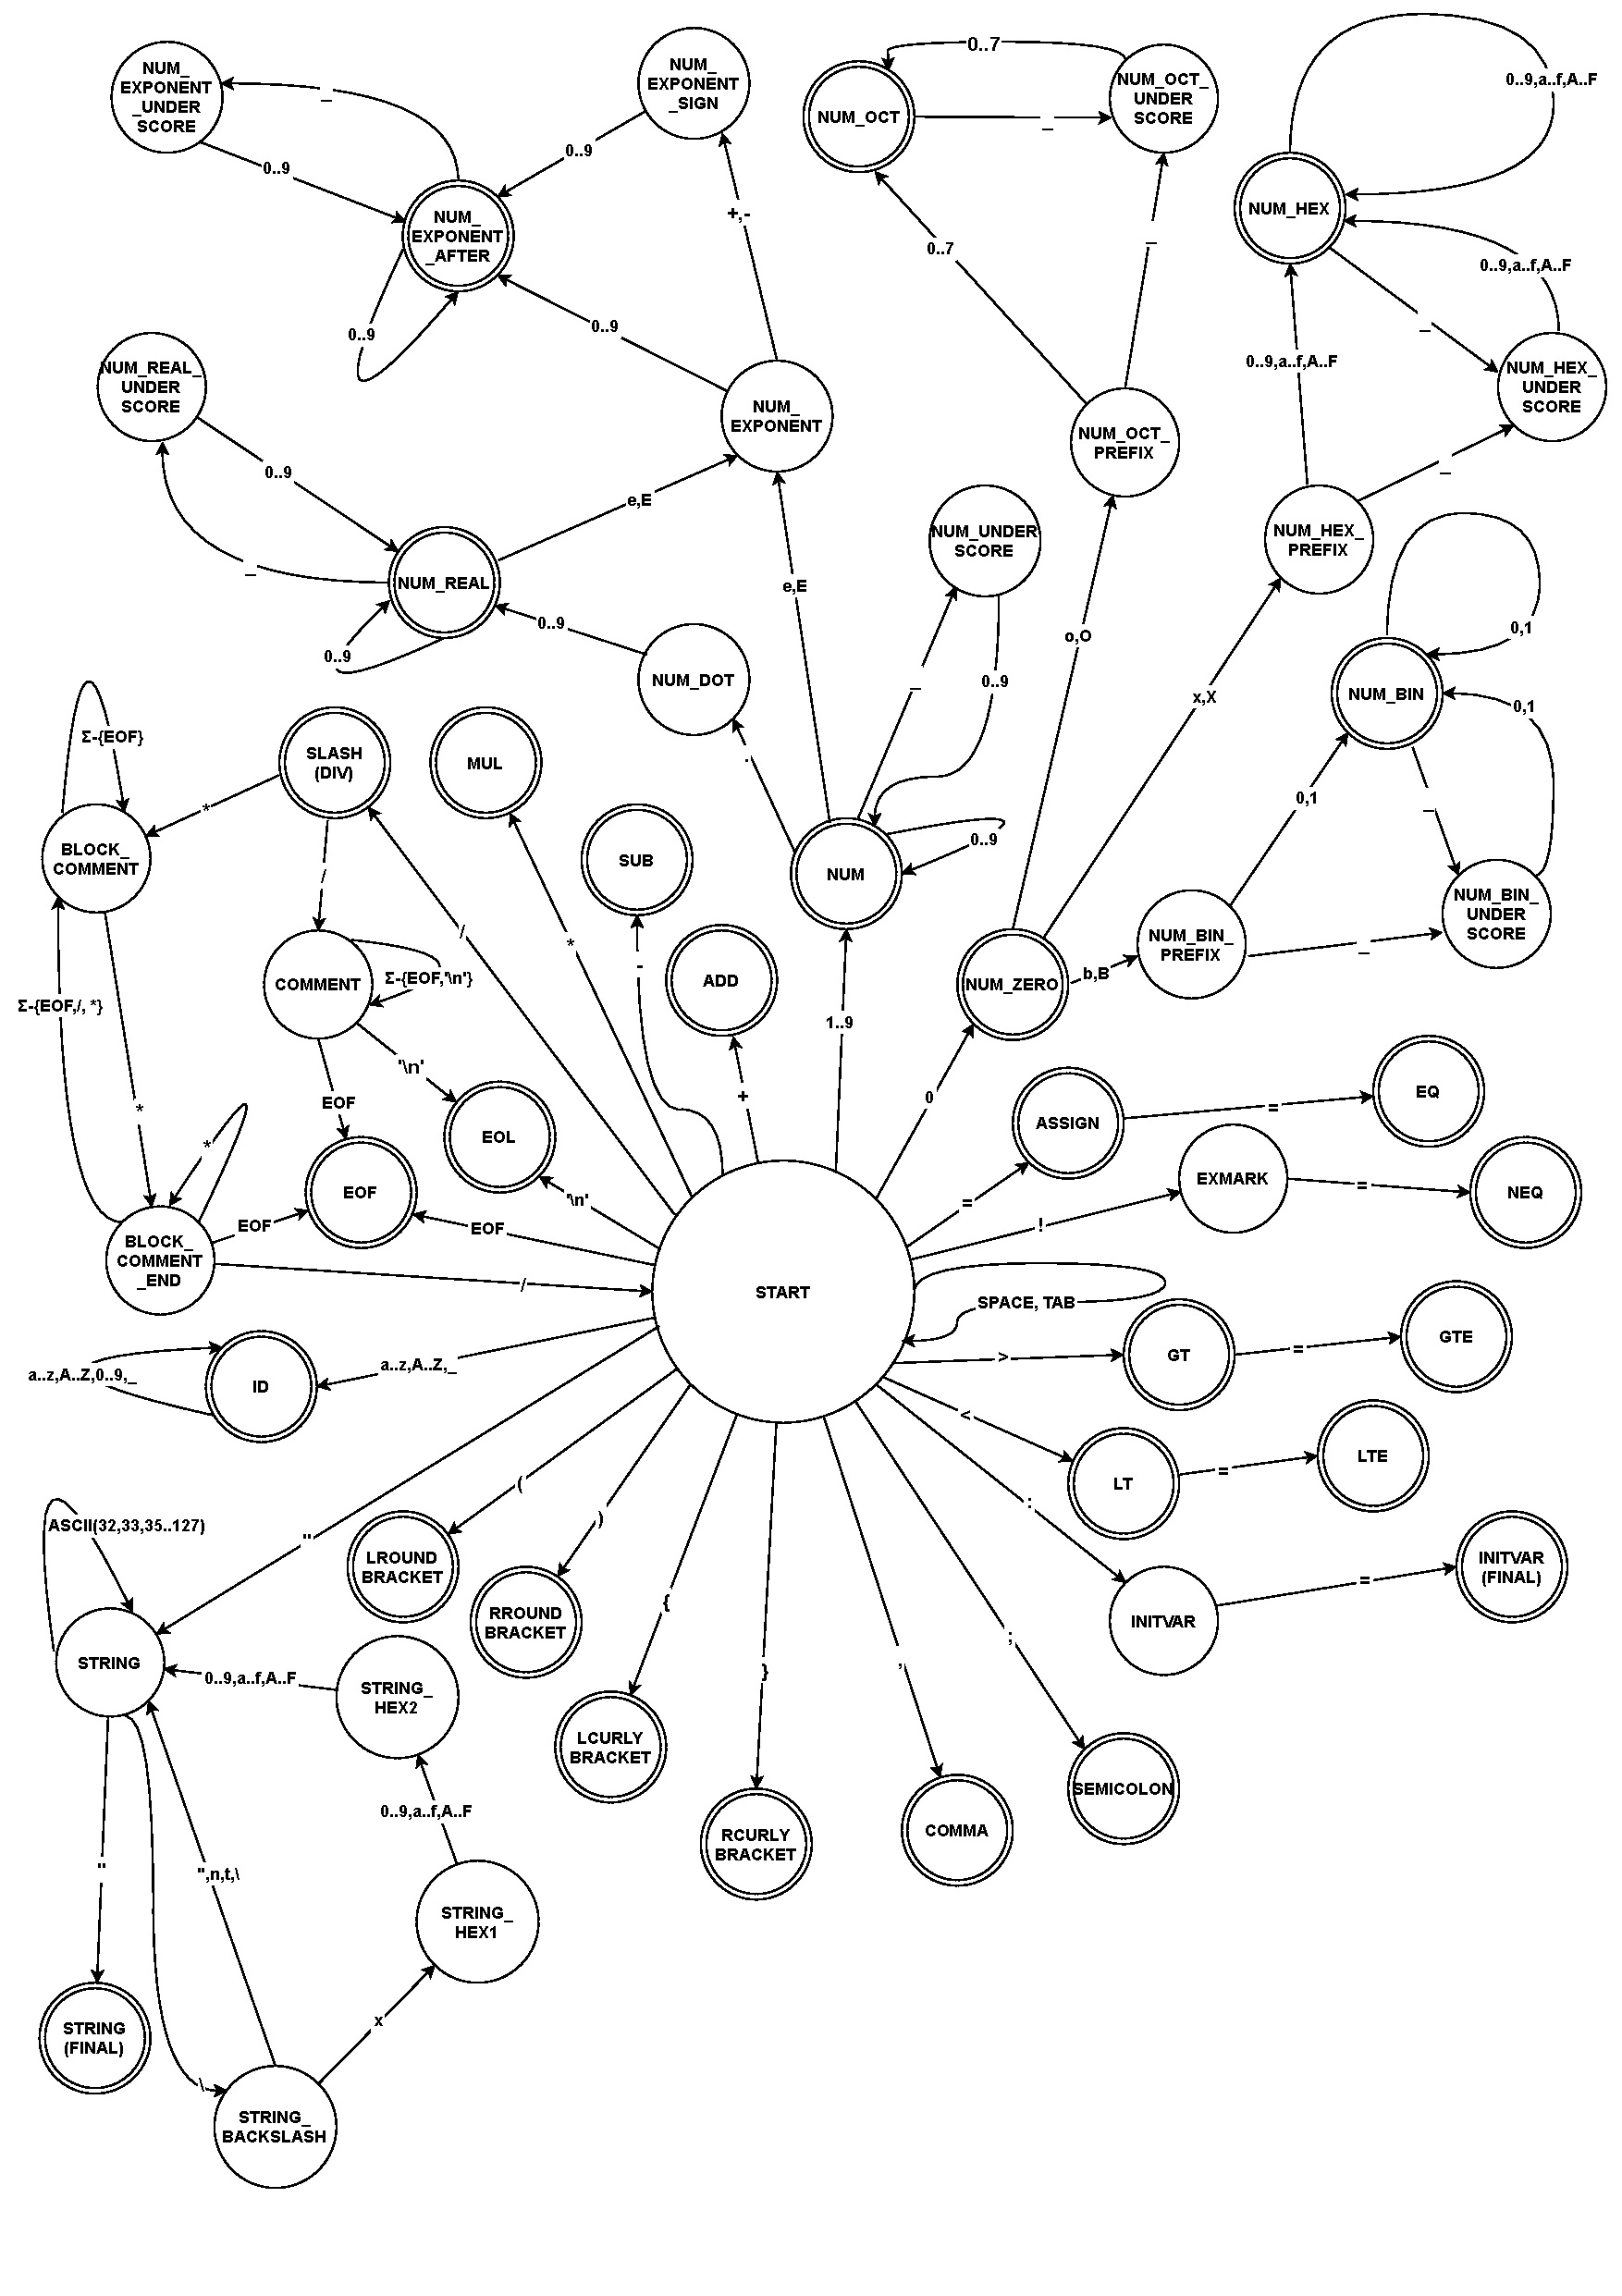
\includegraphics[width=\textwidth,height=\textheight,keepaspectratio]{Scanner_FSM_Graph.pdf}

\newpage

\section{Syntaktická analýza}
Prediktivní syntaktická analýza
    
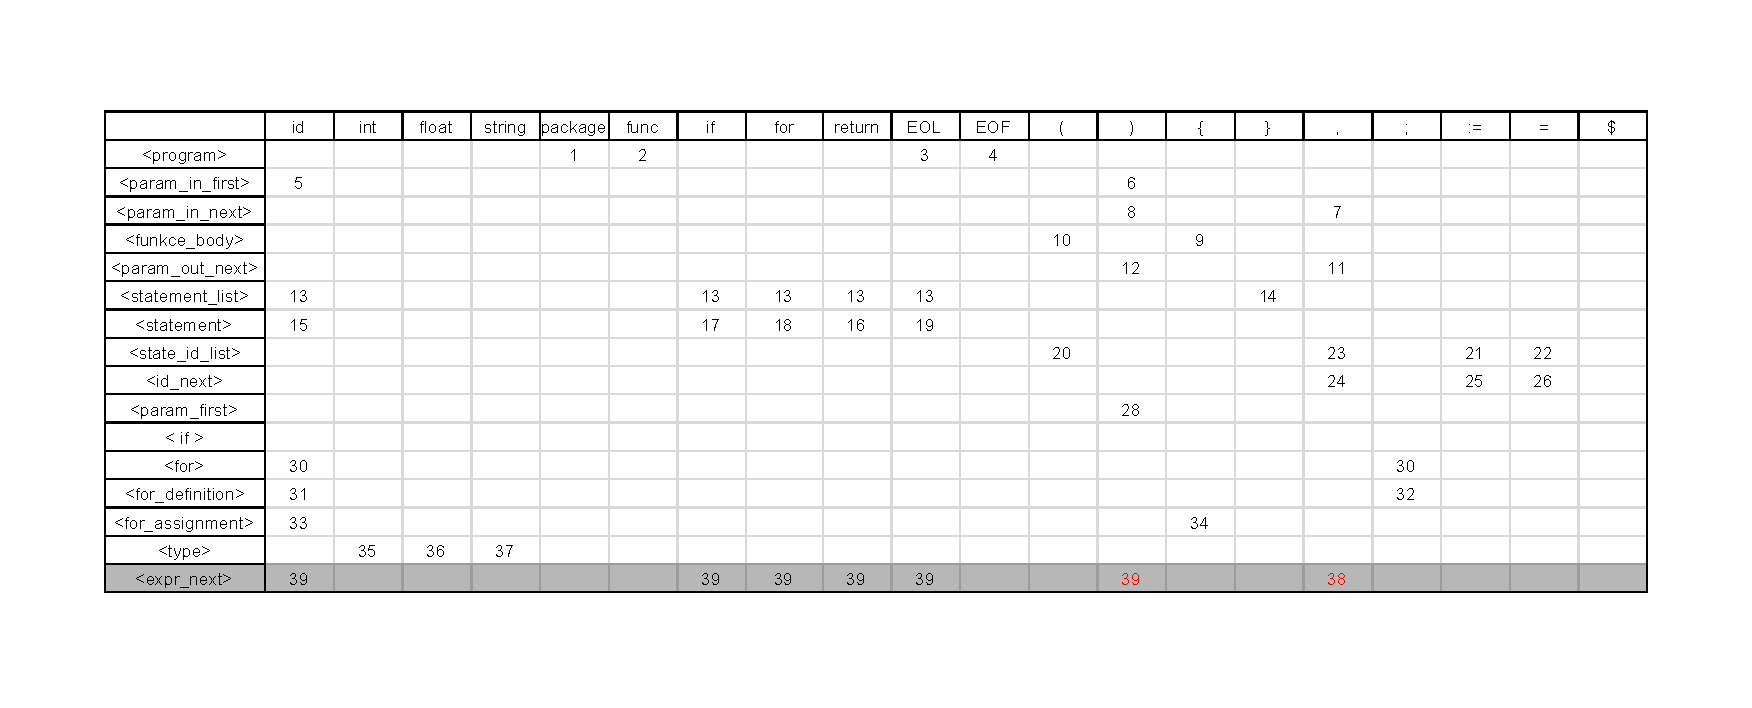
\includegraphics[width=\textwidth,keepaspectratio]{LL_table.pdf}

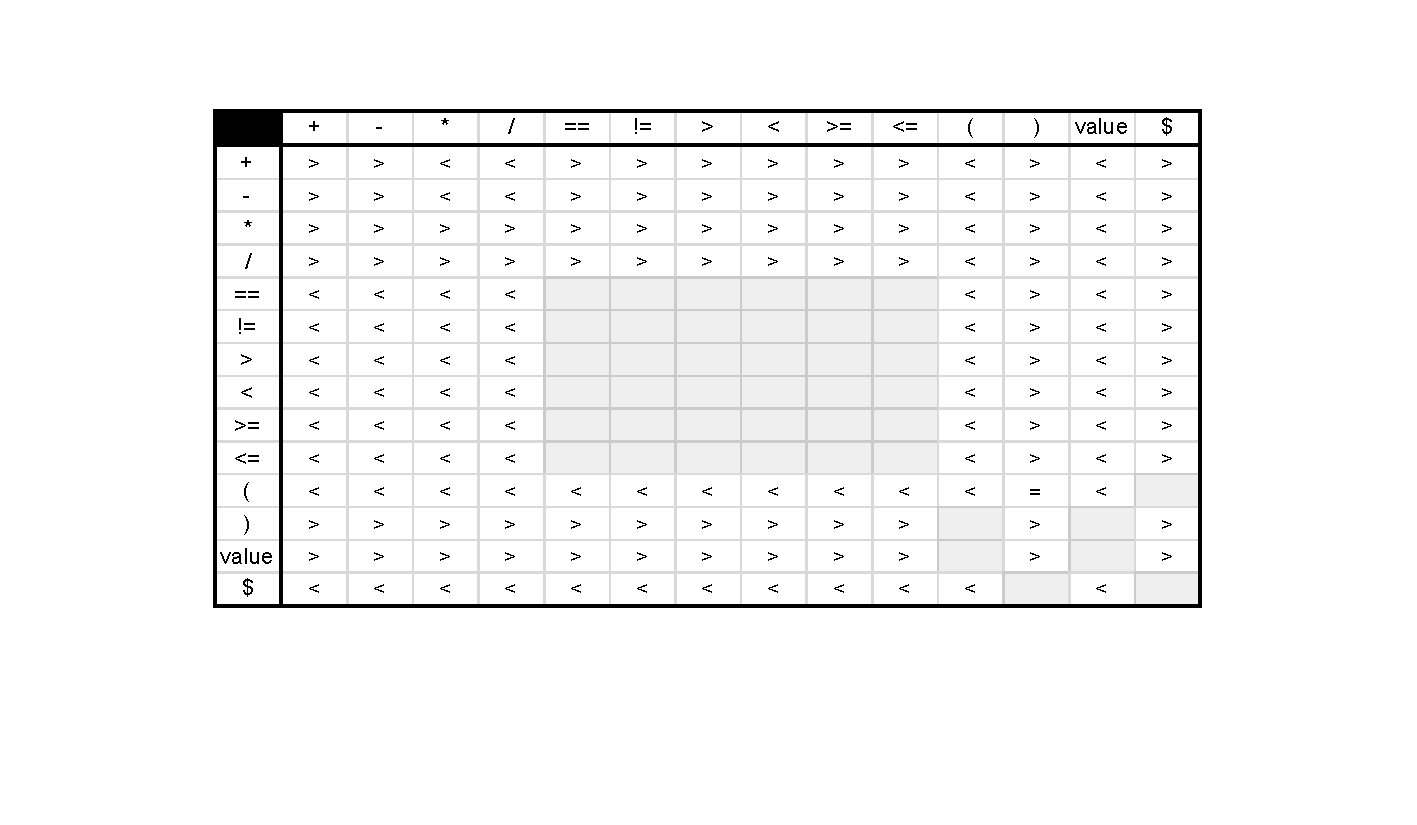
\includegraphics[width=\textwidth,keepaspectratio]{Precedence_table.pdf}


\newpage

\subsection{LL -- gramatika}

		\begin{enumerate}[noitemsep]
		
            \item \verb|<program> -> package id EOL <program>| 
            \item \verb|<program> -> func id ( <param_in_first> ) <func_body> <program>|
            \item \verb|<program> -> EOL <program>|
            \item \verb|<program> -> EOF |
            
            \item \verb|<param_in_first> -> id <type> <param_in_next> |
            \item \verb|<param_in_first> ->| $\varepsilon$
            \item \verb|<param_in_next> -> , id <type> <param_in_next>|
            \item \verb|<param_in_next> -> | $\varepsilon$
            
            \item \verb|<func_body> -> { EOL <statements> }|
            \item \verb|<func_body> -> ( <type> <param_out_next> ) { EOL <statements> } |
            
            \item \verb|<param_out_next> -> , <type> <param_out_next> |
            \item \verb|<param_out_next> ->| $\varepsilon$
            
            \item \verb|<type> -> int|
            \item \verb|<type> -> float| 
            \item \verb|<type> -> string|
            
            \item \verb|<statements> -> id <statement_id> EOL <statements>|
            \item \verb|<statements> -> return EXPRESSION <expr_next> EOL <statements>|
            \item \verb|<statements> -> if EXPRESSION { EOL <statements> }|\newline \verb|                else { EOL <statements> } EOL <statements>|
            \item \verb|<statements> -> for <for_definition> ; EXPRESSION ; <for_assignment>|\newline \verb|                { EOL <statements> } EOL <statements>|
            \item \verb|<statements> -> EOL <statements>|
            \item \verb|<statements> ->| $\varepsilon$
            
            \item \verb|<statement_id> -> ( <arg_first> )|
            \item \verb|<statement_id> -> := <id_expression>|
            \item \verb|<statement_id> -> = <id_expression>|
            \item \verb|<statement_id> -> , id <id_next>|
            
            \item \verb|<id_next> -> , id <id_next>|
            \item \verb|<id_next> -> = <ids_expression>|
            
            \item \verb|<for_definition> -> id := <ids_expression>|
            \item \verb|<for_definition> -> | $\varepsilon$
            
            \item \verb|<for_assignment> -> id := <for_assign_id>|
            \item \verb|<for_assignment> -> | $\varepsilon$
            \item \verb|<for_assign_id> -> , id <for_assign_id>|
            \item \verb|<for_assign_id> -> = <ids_expression>|
            
            \item \verb|<id_expression> -> id ( <arg_first> )|
            \item \verb|<id_expression> -> <expr>|
            
            \item \verb|<ids_expression> -> id ( <arg_first> )|
            \item \verb|<ids_expression> -> <expr> <expr_next>|
            
            \item \verb|<expr_next> -> , <expr> <expr_next>|
            \item \verb|<expr_next> ->| $\varepsilon$
        
            \item \verb|<arg> -> INT|
            \item \verb|<arg_first> -> INT <arg_next>|
            \item \verb|<arg_first> -> FLOAT <arg_next>|
            \item \verb|<arg_first> -> STRING <arg_next>|
            \item \verb|<arg_first> -> id <arg_next>|
            \item \verb|<arg_first> ->| $\varepsilon$
           
            \item \verb|<arg_next> -> , <arg> <arg_next>|
            \item \verb|<arg_next> ->| $\varepsilon$
            \item \verb|<arg> -> FLOAT|
            \item \verb|<arg> -> STRING|
            \item \verb|<arg> -> id| 
            
            
            
        \end{enumerate} 
\newpage

\section{Semantická analýza}
Běží zároveň se syntaktickou TODO

\newpage

\section{Tabulka symbolů}

\newpage

\section{Generace mezikódu}
Generování cílového kódu IFJcode20 probíhá paralelně se syntaktickou a sémantickou analýzou. Parser generátoru předává sekvenci pravidel LL tabulky pravého a levého rozboru, list tokenů z lexikálního analyzátoru , sémantický stack, který obsahuje tokeny na generování výrazu. Hlavní funkcí je \verb|generatorGenerateCode|, která tiskne instrukce prostřednictvím přepínače \verb|switch| a instrukce aritmetických a logických operací prostřednictvím podmíněného cyklu \verb|while| za pomocí sémantického zásobníku předávaného parserem.\\
\newline
Ke generování podmíněných příkazů \verb|if| je použit zásobník na ukládání celočíselných hodnot, které reprezentují jednotlivé ID daných podmíněných příkazů, kvůli správnému výpisu návěští \verb|LABEL| pro \verb|if| a \verb|else|. \\
\newline
Tisk instrukcí probíhá paralelně s parserem na standardní výstup.

\newpage

\section{Hlavní funkce main}
Funkce main inicializuje 
\end{document}
